\chapter{Methodology for Geometry Reconstruction}

This chapter presents the methodology to reconstruct the geometry of the scene. In \cref{section:point-registration}, the laser scans of each acquisition are transformed into point clouds. In \cref{section:laser-extrinsic-calibration}, two calibration methods, one of which was developed in this work, are described to obtain the extrinsic calibration of the laser scanner. \cref{section:normal-estimation} describes a method to estimate the normals, based on the structure of the point cloud. In \cref{section:acquisition-registration}, a method to find the transformations between acquisitions is described, to merge the acquisitions into one point cloud. Finally, in \cref{section:filters}, three point cloud filters used in this work are described.

\section{Point Registration}
\label{section:point-registration}

Each laser scan is a collection of points in polar coordinates, so each range point $(r_i, \theta_i)$ is transformed to a point in the laser frame of reference according to \cref{eqn:range-to-point}. The angles are uniform distributed between a minimum and maximum angle, $\theta_{min}$ and $\theta_{max}$, respectively, so $\theta_i = \{\theta_{min}, \ \dots, \ \theta_{max}\}, i=1 \dots N$. The index $i$ is defined as the range index of each laser scan.

\begin{equation}\label{eqn:range-to-point}
    \left[
        \begin{array}{c}
            x_i \\
            y_i \\
            z_i \\
        \end{array}
    \right]
    =
    \left[
        \begin{array}{c}
            r_i \cos(\theta_i) \\
            r_i \sin(\theta_i) \\
            0 \\
        \end{array}    
    \right]
\end{equation}

Further on, each point $p_{ij}$ is registered in the referencial of the acquisition. According to the transformation graph (see \cref{figure:geometric-transformation-graph}), there are two transformation from the acquisition frame and the laser scanner frame: the transform from the acquisition frame to the PTU frame $\TF{acq}{ptu}$, which is dynamic and depends on the PTU position for each laser scan, and the transformation from the PTU frame and the laser scanner frame $\TF{ptu}{laser}$, which is static. This two transformations can be chained together to obtain the point in the acquisition frame, according to:


\begin{figure}
    
    \centering
    \begin{tikzpicture}
        % \node[draw, ellipse] (scene) {$scene$};
        % \node[draw, ellipse, right of=scene, xshift=3cm] (acquisition) {$acquisition$};
        % \node[draw, ellipse, right of=acquisition, xshift=3cm] (ptu) {$PTU$};
        % \node[draw, ellipse, right of=ptu, xshift=2cm] (laser) {$laser$};
        
        % \draw[-latex] (scene) -- (acquisition)
        % node[midway, above] {$\TF{scene}{acq}$};
        % \draw[-latex] (acquisition) -- (ptu)
        % node[midway, above] {$\TF{acq}{ptu}$};
        % \draw[-latex] (ptu) -- (laser)
        % node[midway, above] {$\TF{ptu}{laser}$};

        \tikzset{
            frame/.style={draw, ellipse, minimum width=3cm},
        }

        \node[frame] (scene) at (0,0) {scene};
        \node[frame] (acquisition) at (0, -2) {acquisition};
        \node[frame] (ptu) at (0, -4) {PTU};
        \node[frame] (camera) at (3, -6) {camera};
        \node[frame] (laser) at (-1, -8) {laser scanner};

        \draw[-latex] (scene) -- (acquisition)
            node[midway, right] {$\TF{scene}{acquisition}$};
        \draw[-latex] (acquisition) -- (ptu)
            node[midway, right] {$\TF{acquisition}{PTU}$};
        \draw[-latex] (ptu) -- (camera)
            node[midway, right] {$\TF{PTU}{camera}$};
        \draw[-latex, blue] (ptu) -- (laser)
            node[midway, below right] {$\TF{PTU}{laser}$};
        \draw[-latex, red] (camera) -- (laser)
            node[midway, right] {$\TF{camera}{laser}$};
    \end{tikzpicture}
    
    \caption{Transformation graph.}
    \label{figure:geometric-transformation-graph}
\end{figure}

\begin{equation}\label{eqn:point-registration}
    p_{i,j} = 
    \left[
        \begin{array}{c}
            x_{i,j} \\ y_{i,j} \\ z_{i,j} \\ 1 \\
        \end{array}    
    \right]
    =
    \TF{acq}{ptu}
    \cdot \TF{ptu}{laser}
    \cdot
    \left[
        \begin{array}{c}
            r_i \cos(\theta_i) \\
            r_i \sin(\theta_i) \\
            0 \\
            1 \\
        \end{array}    
    \right]
\end{equation}

At this phase, each point has 2 indexes, one for the laser scan index $j=1\dots L$ and another for the range index $i=1\dots N$, relative to the each laser scan. Therefore, at this stage, each point can be indexed with a pair of $(i,j)$ indexes. This point clouds are called structured point clouds.

This reconstruction phase depends heavily on the transformation from the PTU to the laser scanner. This transformation is obtained by a calibration process and is commonly referred to as the extrinsic calibration of the laser scanner.

In conclusion, for each acquisition results a point cloud with $L \times N$ points, where $L$ are the number of laser scans and $N$ the number of range values in each laser scan. Each point can be indexed in a bidimensional space, which is useful for subsequent algorithms.

\section{Laser Extrinsic Calibration}
\label{section:laser-extrinsic-calibration}


\section{Normal Estimation}
\label{section:normal-estimation}

As part of the reconstruction work, it is common to create a mesh using the point cloud, through a process called triangulation. Despite that in this work, this was not performed, it can be done in posterior work. Surface normals are a important property of geometric surfaces and are a requirement for most triangulation algorithms. Also, normals are required for lightning calculation, which can improve the rendering of a point cloud model\footnote{See "Estimating Surface Normals in a PointCloud" in \url{http://pointclouds.org/documentation/tutorials/normal_estimation.php}.}. As an example, the Stanford Bunny model\footnote{From \url{https://www.cc.gatech.edu/~turk/bunny/bunny.html}.} rendered with and without lightning are show in \cref{figure:bunny-normals}. As can be seen, lightning can improve the perception of the geometry of the point cloud model.

Normal estimation is quite trivial for surfaces, but for point clouds the process is quite not as easy. Usually there are two ways to estimate the normals: either by meshing the surface first, and then calculate the normals for the mesh, or using the point cloud itself to infer the normals. However, most meshing algorithms already require the normals to achieve a good result, so the latter option is more effective.

\begin{figure}[h]
    
    \centering
    \begin{subfigure}{0.4\textwidth}
        \centering
        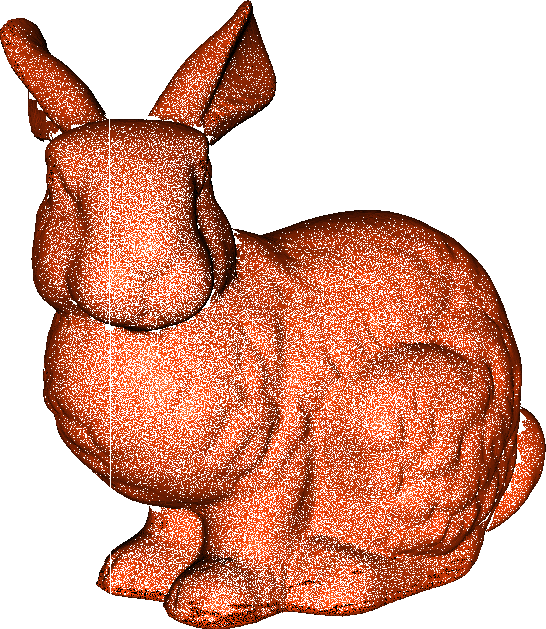
\includegraphics[height=6cm]{bunny-with-normals}     
    \end{subfigure}%
    \begin{subfigure}{0.4\textwidth}
        \centering
        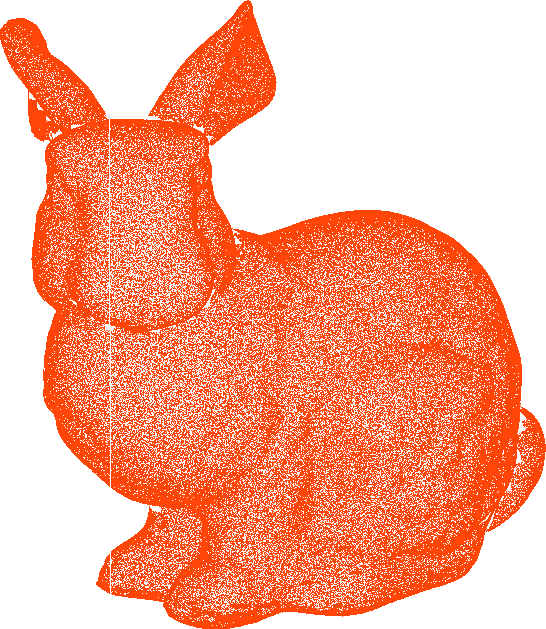
\includegraphics[height=6cm]{bunny-without-normals}     
    \end{subfigure}

    \caption{Stanford rabbit rendering with lightning (on the left), using the normals information, and without lightning (on the right).}
    \label{figure:bunny-normals}

\end{figure}

The most common solution is, for each point, to find the $k$ closest points, defined as the $k$-neighborhood of a point, and calculate the normal of the best-fitting plane formed by this points. However, finding the $k$-neighborhood of all the points in a point cloud has a time complexity $O(N \log N)$, so it can become quite slow for point clouds with a large number of points. In this work, an alternative solution was used to find the closest points, exploiting the bidimensional structure of the point cloud. This solution has a linear time complexity $O(N)$, which makes it a valuable solution for large point clouds.

The solution uses the fact that each point in the point cloud resulting from \cref{section:point-registration} has two indexes, one for the range index $i$ and one for the laser scan $j$. For each laser scan, each point $p_i$ has a neighborhood ${p_{i-k}, \ \dots, \ p_{i+k}}$, because each subsequent point has an increasing angle to the previous point. Between successive laser scans each point has an increasing angle (the pan angle) to the previous one. Therefore, for this algorithm, the neighborhood of each point: 

\begin{equation}
\label{eqn:point-neighborhood}
    neighborhood(p_{i,j}, k_1, k_2) = \{p_{i-k_1, j-k_2}, \ \dots, \ p_{i+k_1, j+k_2}\}.
\end{equation}

\noindent
The value of $k_1$ and $k_2$ have to be adjusted for a better result, because if the values are large, fine details are going to disappear and edges are going to be smeared, and on the other hand if the values are small, the surface will appear as too noisy. In this work, the value of $k_1$ and $k_2$ was 3, so the neighbor has 9 points.

Then, for each point, the tangent plane that fits the neighborhood is calculated, which in turn is a least-square plane fitting problem. This is usually solved by an analysis of Principal Component Analysis, as explained in \cref{section:calibration-cost-function}. This method will compute the direction of the normal $n$ for each point.

Then, the orientation of the point has to be defined, because the result of the PCA is ambiguous, which may lead to inconsistent normals in the point cloud. In this case, the solution found was to orientate the normals towards the frame of the 3D scanner, which for each acquisition in the origin of the coordinate system. Therefore, each normal has to satisfy:

\begin{equation}
\label{eqn:normal-orientation}
    n \cdot p < 0.
\end{equation}

\section{Acquisition Registration}
\label{section:acquisition-registration}

During an acquisition multiple acquisitions are done and to each one corresponds a transformation (position and orientation) to the scene referencial. In this section, a method is described to find each one of this transformations, so all the acquisitions are merged into a single point cloud. The method chosen is the ICP or Iterative Closest Point. This method is capable of aligning two point clouds, the reference and the target point cloud, by finding the transformation between the second to the first one. This is also known as point cloud registration.

\subsection{ICP}

This method can formally be described as follows: let $P$ be the target point cloud and $Q$ the reference point cloud. Then, the aim of the registration is to estimate the transformation $T$ from the referencial of $P$ to $Q$ by minimizing the error function $error(P, Q)$ in \cref{eqn:icp-transformation-function}, where $T(P)$ is the result of the application of the transformation $T$ to the point cloud $P$.

\begin{equation}
\label{eqn:icp-transformation-function}
    T = \underset{T}{argmin}(error(T(P), Q))
\end{equation}

The error function $error(P, Q)$ is computed on pair of points that are associated between the two point clouds. This association is, ideally, between points that are closest in position in both point clouds. Then, the distance between the matching points $(p_i, q_i)$ are used in the error function in \cref{eqn:icp-error-function}. The matching algorithm can be based on features or geometric properties, so a better matching can be found. In this work, a simple point-to-point matching.

\begin{equation}
\label{eqn:icp-error-function}
    error(P, Q) = \sum_{(p_i, q_i)}{|p_i - q_i|}
\end{equation}

In order to make the error function more robust, outlier points can be removed first from the match list. In addition, weights $w_i$ can be associated to each matching points $(p_i, q_i)$ to increase or decrease the influence of each matching points in the error function. As an example, normals can be used as a weight, so points with similar normals ($w_i = n_{p_i} \cdot n_{q_i}$) have a greater influence in the error function. 

However, the result of this minimization is always always dependant on the association between the points, which, unless the descriptors are good enough (like visual correspondences), the matching is not perfect, and is worst the farther apart both point clouds are. The idea behind the ICP algorithm is that, even with a bag association, the resulting estimate can be used to find a better one. So, the ICP algorithm creates a series of transformation $T_i$ at each iteration, yielding a new transformed point cloud $P_i$. Then, the next transformation is found:

\begin{equation}
    T_{i+1} = \underset{T}{argmin}(error(T_i(P_i), Q))
\end{equation}

Finally, the final transformation estimate is the composition of all the intermediary transformations:

\begin{equation}
    T = T_1 \circ T_2 \circ \dots \circ T_N
\end{equation}

\subsection{Multiple Point Cloud ICP}
\label{section:multiple-pointcloud-icp}

However, ICP can only register pairs of point clouds, whereas this work requires a registration of $N$ point clouds, corresponding to $n$ acquisitions. So, a technique has to be found so that the ICP algorithm can be used with $n$ point clouds. Three of this such techniques are now describes, ordered by their complexity.

The first approach and the easier one to implement is to register each point clouds sequencially. In other words, this method registers the point cloud $P_i$ to the point cloud $P_{i-1}$ and the transformation $T_{i-1}^{i}$ is found. The final accumulated point cloud is assembled using the \cref{eqn:registration-simple-method-calculation}. This method is the one that requires less overall registration, but has the downside that the transformation errors increases for each successive point cloud. This approach is shown in \cref{figure:multiple-icp-method-1}.

\begin{equation}
\label{eqn:registration-simple-method-calculation}
    P = \bigcup{\left(T_1^2 \circ T_2^3 \circ \dots \circ T_{i-1}^i\right)(P_i)}
\end{equation}

The next approach is widely used in robotics for Simultaneous Location and Mapping (SLAM). This method holds an accumulated point cloud $A$ in memory, and each new incoming point cloud $P$ registers to the accumulated point cloud and afterwards it is merged into $A$, which is then used for the next iteration, as shown in \cref{figure:multiple-icp-method-2}. It has the advantage that each new registration is done against a wider point cloud and has a smaller influence than in the previous method. Also, at each iteration the current pose of the 3D scanner is obtained, which is used as an initial estimate for the next iteration. However, the accumulated point cloud grows at each iteration, so a down-sampling is done at each iteration to keep the number of points bounded. In conclusion, each iteration can be calculated as:

\begin{align}
    T_{i} = & ICP(A, P_{i}, T_0 = T_{i-1}) \\
    A_{i+1} = & A{i} \bigcup T_{i}(P_i)
\end{align}

The last approach is the most complex. The idea of this approach is to minimize the number of transformation combinations, to minimize the propagation of the error. In particular, the registrations for the $N$ points clouds are done pairwise and are merged together to create $N/2$ point clouds. Then, this process is done recursively until an unique point cloud is obtained. This way, the maximum number of transformation combinations are equal to the number of levels of the tree, which is $\log_2(N)$, instead of $N$ combinations in the first approach. This algorithm is formalized in \cref{eqn:registration-tree-method-1,eqn:registration-tree-method-2}, for a list of point clouds $S=\left\{P_1, P_2, \ \dots, \ P_n\right\}$. At each level $l$ a new list of point clouds $^{l}P$ and transformations $^{l}T$ are computed, as shown in \cref{figure:multiple-icp-method-3}.

\begin{align}
    ^{l}T = & \left\{ICP(^{l-1}P_1, ^{l-1}P_2), \ \dots, \ ICP(^{l-1}P_{n-1}, ^{l-1}P_{n}) \right\}
        \label{eqn:registration-tree-method-1} \\
    ^{l}P = & \left\{^{l-1}P_1 \bigcup{^{l}T_1(^{l-1}P_2}), \ \dots, \ ^{l-1}P_{n-1} \bigcup{^{l}T_{n/2}(^{l-1}P_n)}\right\}
        \label{eqn:registration-tree-method-2}
\end{align}

In conclusion, three methods are possible to extend the ICP algorithm to multiple point clouds. After all the registrations are performed, point cloud can be assembled from all the point clouds, to form a big point cloud of the final scene. There is, however, a limitation of all this methods, because all of them have the principle that every point cloud is close to the previous one, which can be false. In this work, this was ensured in the capture methodology. 

\begin{figure}
    \centering
    \begin{subfigure}[t]{0.3\textwidth}
        \centering
        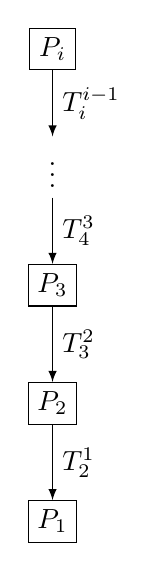
\begin{tikzpicture}
            \node[draw] (P1) at (0,0) {$P_1$};
            \node[draw] (P2) at (0,1.5) {$P_2$};
            \node[draw] (P3) at (0,3) {$P_3$};
            \node (P4) at (0,4.5) {$\vdots$};
            \node[draw] (Pi) at (0,6) {$P_i$};

            \draw[-latex] (P2) -- (P1) node[midway, anchor=west] {$T_2^1$};
            \draw[-latex] (P3) -- (P2) node[midway, anchor=west] {$T_3^2$};
            \draw[-latex] (P4) -- (P3) node[midway, anchor=west] {$T_4^3$};
            \draw[-latex] (Pi) -- (P4) node[midway, anchor=west] {$T_i^{i-1}$};
        \end{tikzpicture}

        \caption{First method}
        \label{figure:multiple-icp-method-1}
    \end{subfigure}%
    \begin{subfigure}[t]{0.3\textwidth}
        
        \centering
        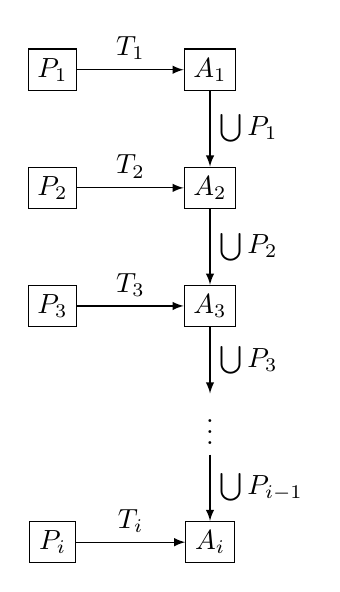
\begin{tikzpicture}
            \node[draw] (A1) at (0,0) {$A_1$};
            \node[draw] (A2) at (0,-1.5) {$A_2$};
            \node[draw] (A3) at (0,-3) {$A_3$};
            \node (A4) at (0,-4.5) {$\vdots$};
            \node[draw] (Ai) at (0,-6) {$A_i$};

            \node[draw, left of=A1, xshift=-1cm] (P1) {$P_1$};
            \draw[-latex] (P1) -- (A1) node[midway, above] {$T_1$};

            \node[draw, left of=A2, xshift=-1cm] (P2) {$P_2$};
            \draw[-latex] (P2) -- (A2) node[midway, above] {$T_2$};

            \node[draw, left of=A3, xshift=-1cm] (P3) {$P_3$};
            \draw[-latex] (P3) -- (A3) node[midway, above] {$T_3$};

            \node[draw, left of=Ai, xshift=-1cm] (Pi) {$P_i$};
            \draw[-latex] (Pi) -- (Ai) node[midway, above] {$T_i$};

            \draw[-latex] (A1) -- (A2) node[midway, right] {$\bigcup{P_1}$};
            \draw[-latex] (A2) -- (A3) node[midway, right] {$\bigcup{P_2}$};
            \draw[-latex] (A3) -- (A4) node[midway, right] {$\bigcup{P_3}$};
            \draw[-latex] (A4) -- (Ai) node[midway, right] {$\bigcup{P_{i-1}}$};
        \end{tikzpicture}

        \caption{Second method}
        \label{figure:multiple-icp-method-2}
    \end{subfigure}%
    \begin{subfigure}[t]{0.4\textwidth}
        
        \centering
        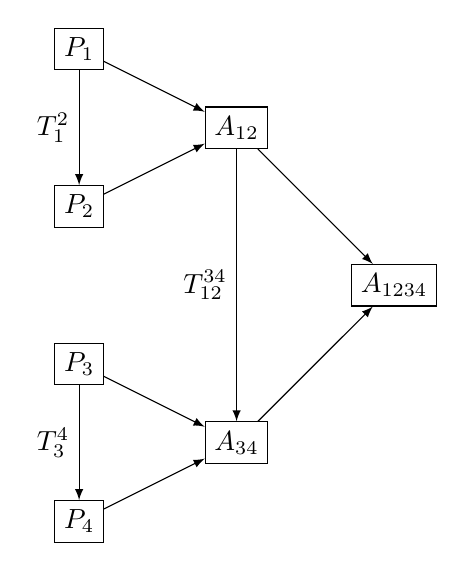
\begin{tikzpicture}
            \node[draw] (P1) at (0,0) {$P_1$};
            \node[draw] (P2) at (0,-2) {$P_2$};
            \node[draw] (P3) at (0,-4) {$P_3$};
            \node[draw] (P4) at (0,-6) {$P_4$};

            \node[draw] (A12) at (2, -1) {$A_{12}$};
            \node[draw] (A34) at (2, -5) {$A_{34}$};
            \node[draw] (A1234) at (4, -3) {$A_{1234}$};

            \draw[-latex] (P1) -- (A12);
            \draw[-latex] (P2) -- (A12);
            \draw[-latex] (P3) -- (A34);
            \draw[-latex] (P4) -- (A34);
            \draw[-latex] (A12) -- (A1234);
            \draw[-latex] (A34) -- (A1234);

            \draw[-latex] (P1) -- (P2) node[midway, left] {$T_1^2$};
            \draw[-latex] (P3) -- (P4) node[midway, left] {$T_3^4$};
            \draw[-latex] (A12) -- (A34) node[midway, left] {$T_{12}^{34}$};

        \end{tikzpicture}
        \caption{Third method}
        \label{figure:multiple-icp-method-3}
    \end{subfigure}%


    \caption{Multiple Point Cloud ICP approaches}
    \label{figure:registration-methods-approaches}
\end{figure}
\section{Filters}
\label{section:filters}

The final point cloud, after the assembly from every acquisition's point cloud, can have unnecessary or redundant information, which can make the point cloud size too large for any use. A common solution is to use filters to remote unnecessary points and downsample the point cloud.

\subsection{NaN Removal}

The first filter is the Not a Number removal, or NaN removal. In the first steps of the reconstruction, the point cloud is stored as a dense point cloud, or structured point cloud. To maintain this structure, NaNs are used to mark the missing values, which are usually originated by measurement errors. When the structure of the point cloud becomes irrelevant, its dimensions are collapsed into one. After, the NaNs become irrelevant and are removed from the point cloud.



In the acquisition, any range that is not measured is stored as a NaN, to signal that they are missing. During the point registration phase, all this missing ranges remain as NaN, and should be removed, because their information is irrelevant and take as much space as a real value. So, each point that contains a NaN value is removed from the final point cloud.

\subsection{Statistic Outlier Removal}

Usually point clouds contains different point densities, dependent on the distance of the object to the sensor. Also, measurement errors also occur next to edges or corners. As a result, point clouds tend to have sparse outliers that can affect subsequent algorithms, like segmentation or registration algorithms. A usual solution is to perform an statistically analysis on each point, removing the ones that do not reach a certain criteria. In particular, the mean distance of each point to its neighbors is computed, and if this distance is outside an interval centered in the mean of all the distances, then it is removed. An example can be seen in \cref{figure:sor-filter}.

\begin{figure}[h]
    
    \centering
    \begin{subfigure}[t]{0.5\textwidth}
        
        \centering
        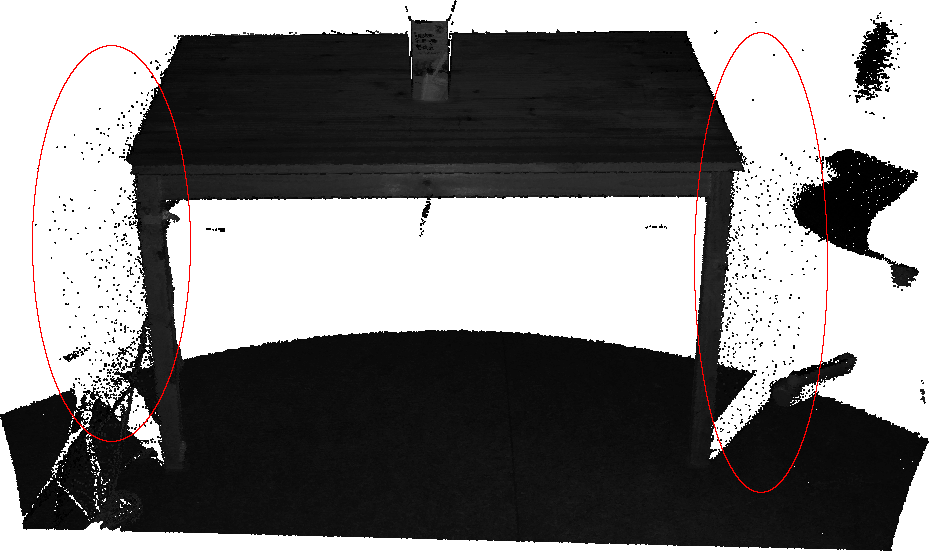
\includegraphics[width=0.8\textwidth]{table-with-outliers}
        \caption{Before SOR}
        \label{figure:sor-filter-before}
    \end{subfigure}%
    \begin{subfigure}[t]{0.5\textwidth}
        \centering
        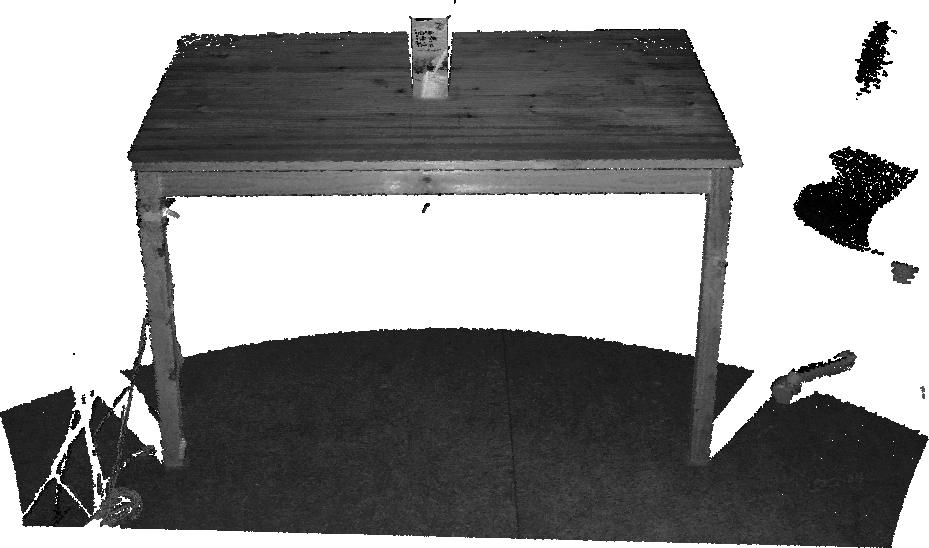
\includegraphics[width=0.8\textwidth]{table-without-outliers}
        \caption{After SOR}
        \label{figure:sor-filter-after}
    \end{subfigure}

    \caption{SOR filter in a point cloud, processed by the software \textit{CloudCompare}.}
    \label{figure:sor-filter}
\end{figure}

\subsection{Voxel Grid Downsampling}

This method downsamples, that is, reduce the number of points of a point cloud, using a voxel grid. A voxel is a cubical space and is the element in a tridimensional grid. So, each point in the point cloud belongs to some voxel. Then, in each voxel, all the points are represented by their centroid. This is an effective and fast method to downsample a point cloud. The level of detail can be parameterized with the voxel leaf-size (the size of each voxel in the $x,y,z$ direction). A smaller leaf-size maintains more details but generates a bigger point cloud. A bigger leaf-size does not keep as much detain but generates a smaller point cloud. As an example, \cref{figure:lucy-voxel-grid} shows the Stanford Lucy model\footnote{From "Stanford Scanning Repository" in \url{graphics.stanford.edu/data/3Dscanrep/}.} after a voxel grid downsampling with different leaf size values: \cref{figure:lucy-voxel-grid-2mm} with \SI{2}{\milli\meter} (288.000~pts), \cref{figure:lucy-voxel-grid-5mm} with \SI{5}{\milli\meter} (55.000~pts) and \cref{figure:lucy-voxel-grid-8mm} with \SI{2}{\milli\meter} (18.000~pts).

\begin{figure}[h]
    
    \centering
    \begin{subfigure}[t]{0.3\textwidth}
        \centering
        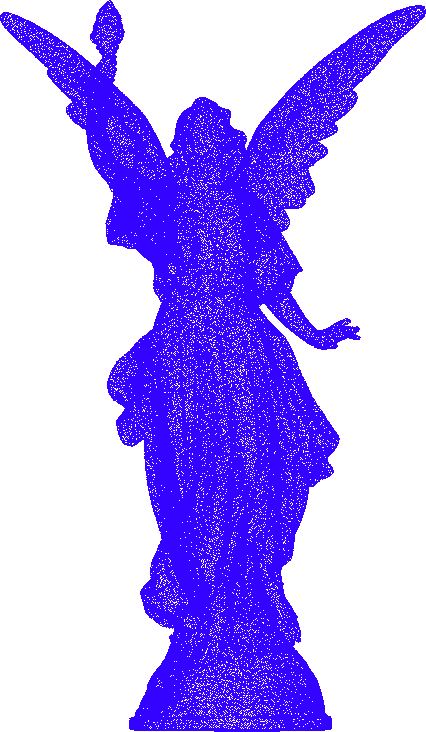
\includegraphics[height=6cm]{lady-voxel-2mm}
        \caption{Leaf size of \SI{2}{\milli\meter}}
        \label{figure:lucy-voxel-grid-2mm}
    \end{subfigure}%
    \begin{subfigure}[t]{0.3\textwidth}
        \centering
        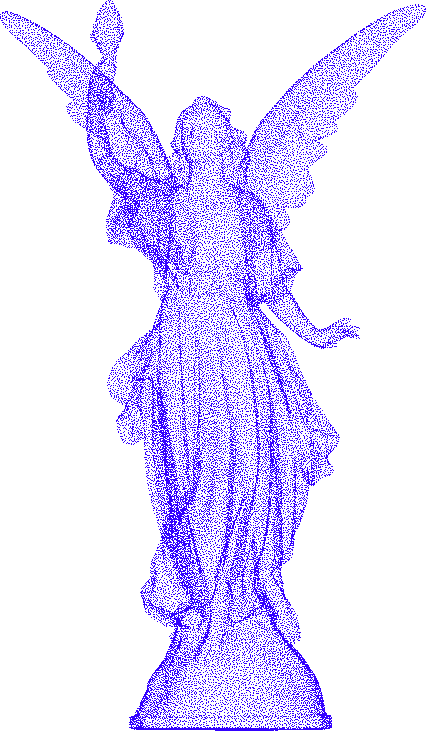
\includegraphics[height=6cm]{lady-voxel-5mm}
        \caption{Leaf size of \SI{5}{\milli\meter}}
        \label{figure:lucy-voxel-grid-5mm}
    \end{subfigure}%
    \begin{subfigure}[t]{0.3\textwidth}
        \centering
        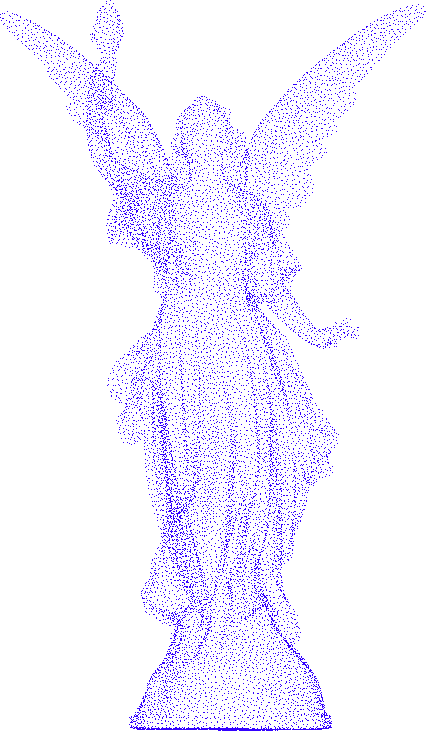
\includegraphics[height=6cm]{lady-voxel-8mm}
        \caption{Leaf size of \SI{8}{\milli\meter}}
        \label{figure:lucy-voxel-grid-8mm}
    \end{subfigure}

    \caption{Stanford Lucy scan after a voxel grid downsampling with different leaf sizes.}
    \label{figure:lucy-voxel-grid}
\end{figure}
